

\documentclass{article}
\usepackage{graphicx}

\title{Computation \& Robot Vision: Lecture 1}
\author{Sam Barrett}

\begin{document}
\maketitle

\section{Camera and image formation}
\label{sec:cif}

\subsection{The human eye}
\label{subsec:human-eye}

The ultimate goal of Computer vision is to allow computers to \textit{see} in a similar (or better) way to humans.

We must first start with what we are trying to emulate: the human eye.

\begin{figure}[ht]
  \centering
  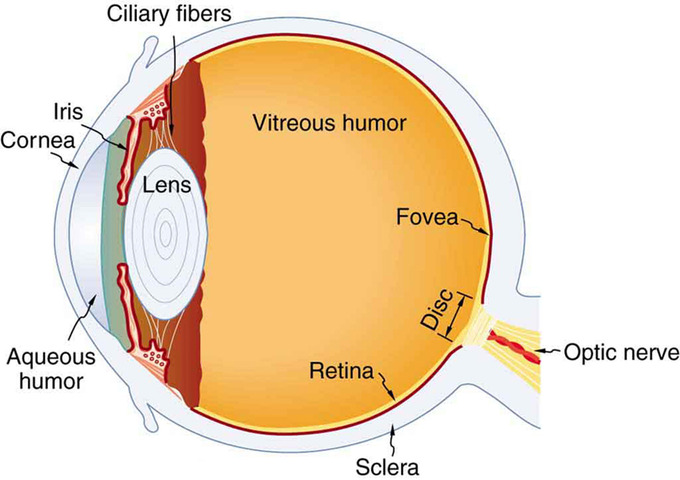
\includegraphics[scale=0.5]{figures/human-eye.jpeg}
  \caption{\label{fig:human-eye} Diagram of the human eye}
\end{figure}

The human eye works by focusing the light entering via the pupil using the lens. This forms an image on the retina.

The retina is made up of many different types of cells, ultimately terminating in the ganglion cells which feed information to the brain via optic nerve fibres. It's composition can be seen in Figure~\ref{fig:retina}.

\begin{figure}[ht]
  \centering
  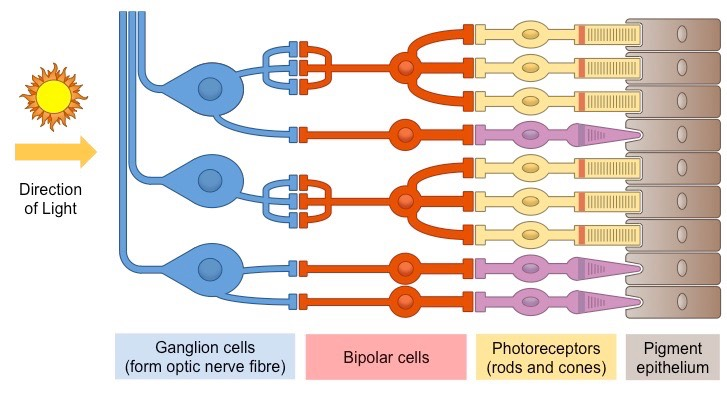
\includegraphics[scale=0.3]{figures/retina_med.jpeg}
  \caption{\label{fig:retina} Diagram of the retina}
\end{figure}

The ganglion cells collect information regarding the visual world from bipolar and amacrine cells. The information takes the form of chemicals messages emitted by receptors on the ganglion cell's membrane.

\subsection{Evolution of cameras}

The evolution of artificial cameras started in the renaissance with the likes of Da Vinci experimenting with camerae obscurae (pinhole image projections) and perspective. Later, photographic film was invented, allowing for the capture of images by exposing the film to different levels of light, focused by a lens the same as we have seen in Figure~\ref{fig:human-eye}.

We have since gone on to develop entirely digital cameras but the principals remain the same. Here, the photographic film containing photosensitive particles is replaced with a camera \textit{sensor} which are arrays of light-sensitive diodes which convert photons to electrons.

\begin{figure}[ht]
  \centering
  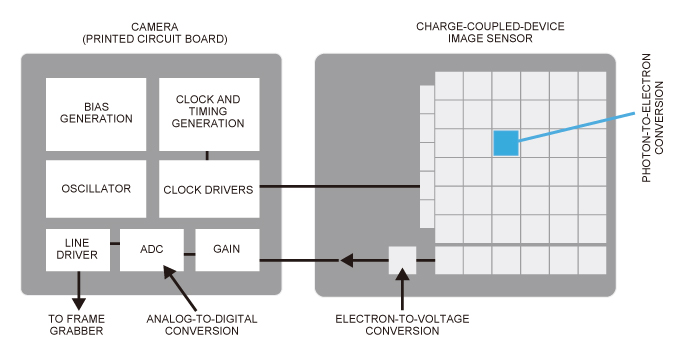
\includegraphics[scale=0.3]{figures/digital-sensor.jpg}
  \caption{\label{fig:digital-sensor} Basic photosensor construction }
\end{figure}

Digital images are a 2D grid (or matrix) of integers which show the continuous fluctuations in levels of light.

\subsubsection{Encoding colour}

How do we encode colour into this matrix of integers? We first need to decide on a representation of colour that a computer can understand. We do this by decomposing colours into their primary components. I.e. the different levels of red, green and blue. We can represent \textbf{any} colour using weighted combinations of these colours.

Unfortunately, each photodiode is \textit{colour blind} and cannot tell the colour of the light hitting it, only it's intensity. So in order to detect the colour of an image, sensors deploy filters such as the Bayer filter. These are layouts of photo-diodes such that each receptor site is known to only detect light from a particular part of the spectrum. The Bayer filter can be seen in Figure~\ref{fig:bayer1}. Using such a filter we can estimate the RGB at each cell using the values of it's neighbours.

\begin{figure}[ht]
  \centering
  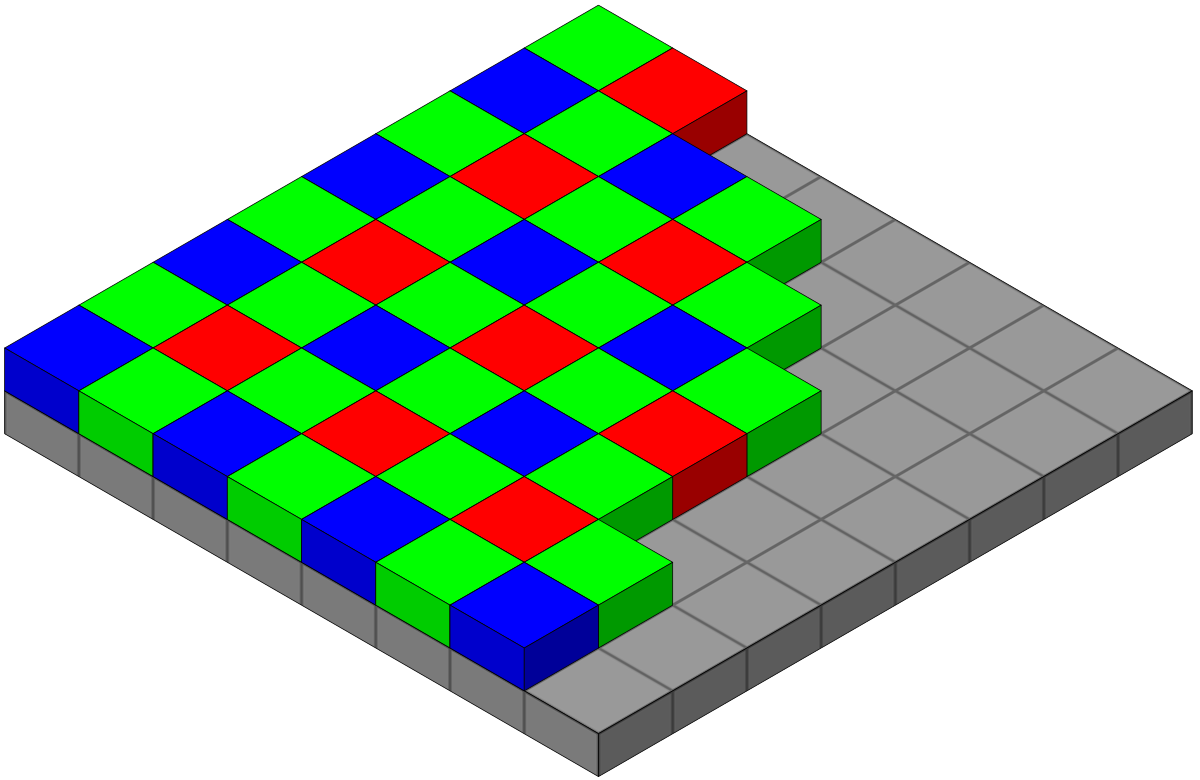
\includegraphics[scale=0.1]{figures/bayer1.png}
  \caption{\label{fig:bayer1} Bayer filter overtop of a sensor}
\end{figure}

\begin{figure}[ht]
  \centering
  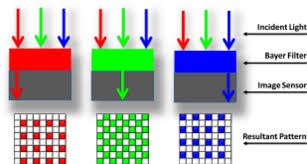
\includegraphics[scale=0.5]{figures/bayer2.jpeg}
  \caption{\label{fig:bayer2} Diagram showing effect of the Bayer filter}
\end{figure}

\textit{Why are there twice as many green as red and blue pixels?}

This is done to mimic the higher sensitivity the human eye has towards green light.


\end{document}

